\documentclass[11pt,a4paper]{article}
\usepackage{theme/lmuthesis}

% this for draft water mark
\setboolean{release}{true}

\ifthenelse{\boolean{release}}{
}{
    \usepackage{draftwatermark}
    \SetWatermarkText{DRAFT}
    \SetWatermarkScale{1}
}

% meta informations
\department{Institut f\"ur Informatik}
\lfe{Lehr- und Forschungseinheit Medieninformatik}
\professor{Prof.\ Dr.\ Andreas Butz}
\type{Bachelor's Thesis}
\title{Progressive BVH Refinement in Interactive Ray Tracing}
\author{Christian Schmidt}
\email{nichtchristianschmidt@gmail.com}
\bearbeitungszeitraum{06.05.2021 bis END}
\supervisor{Changkun Ou}
\taskdescription{
    \begin{description}
        \item[THESIS TITLE]
        \item[Problem Statement] TO BE ADDED
        \item[Scope of the Thesis] TO BE ADDED
        \item[Tasks] TO BE ADDED
        \item[Requirements] TO BE ADDED
        \item[Keywords] TO BE ADDED
    \end{description}
}
\acknoledgement{
    I would like to appreciate ...
}
\abstract{
    This thesis proposes ...
}

\begin{document}

\makecover
\maketaskdescription
\makededication
\makeabstract
\maketoc
% optional:
% \listoffigures
% \listoftables
\cleardoublepage

\section{Introduction}
Ray tracing is foremost a rendering technique simulating how light travels through a scene and thus inherently producing very realistic images. Effects that need to be simulated explicitly in the contrasting approach of rasterization, such as shadows, reflections and refractions are achieved by default, albeit introducing a substantial computational cost. It is this simplicity paired with the high quality output, that made the method a staple in offline rendering where the relatively long rendering time can be tolerated. In real-time settings where the time to render single frames is limited, ray tracing is a rather poor fit and requires a number of optimizations to push its performance to a sufficient point. Only in recent years has that point been reached and surpassed far enough to open the technology up for a consumer market, especially by utilizing special-purpose hardware. A particularly noteworthy milestone in that regard is NVIDIA's Turing architecture\cite{nvidia2017turing}, which is built in a way that accelerates basic ray tracing operations while also facilitating other software technologies essential to the process, most importantly more advanced denoising techniques. However, the availability of such graphic cards is still limited, so software based solutions remain an interesting topic which this thesis tries to tackle. 

% TODO: Add references to the corresponding sections 
In particular, this thesis provides a self-contained overview over the basics of real-time ray tracing as well as some implementation details of an interactive CPU path tracer written from scratch, which might be useful as a starting point for further research and more optimizations. Furthermore, a closer look at bounding volume hierarchies is presented, and the approach of progressive hierarchical refinement\cite{hendrich_parallel_2017} is introduced as a state-of-the-art algorithm to construct such acceleration structures. The integration of the aforementioned approach into an interactive path tracer is described and validated, as this was still an open question. Finally, two methods for optimizing hyperparameters related to the construction algorithm in real-time are introduced, evaluated and discussed.
\section{Related Work}
\label{ch:related}

\epigraph{That men do not learn very much from the lessons of history is the most important of all the lessons that history has to teach.}{Aldous Huxley}

\subsection{History of \LaTeX}

The first release of \LaTeX \cite{lamport1994latex} appeared in 1983 \cite{lamport2007writings}.

\cleardoublepage
\section{Path Tracing}
\subsection{Algorithm}
At the core of any ray tracing approach is the concept of a ray, usually in three-dimensional space. In this work the following representation is used.
\[P(t)=O+td\]
% TODO: Introduce math notation
Where the origin $O$ is some point within the scene space and the direction $d$ is some vector along which the ray travels in a straight line. Points along this line can be described using the distance $t$, with $P(0)=O$ and $P(1)=O+d$. 
% TODO: Add Ray tracing Figure
As illustrated in figure 1, this concept can be used to construct images. Rays are cast into a scene, originating at some common eye point and intersecting each pixel in the image plane to find its corresponding color. The first ray casting algorithm using such a technique was proposed by Appel\cite{appel1968}, only considering primary intersections and shadow rays towards a light source to determine whether a point is illuminated or not. Whitted\cite{whitted_improved_1980} expanded on that approach by introducing an algorithm that, upon finding an object intersection, generates secondary rays influencing the final pixel color. In addition to the previously mentioned shadows, these secondary rays allow rendering of reflections and refractions by recursively casting new rays in the reflection direction and blending all results. 
% TODO: Is it really more common?
A more common approach, especially in film and visual effects\cite{keller2015path_tracing_revolution}, is a closely related concept called path tracing\cite{kajiya_rendering_1986}. Instead of evaluating a single ray per pixel, multiple samples with slight offsets and random scattering are used to more accurately simulate light transport through a scene and approximate the rendering equation also introduced by Kajiya. Path tracing is a global illumination solution and thus produces more realistic results, while also allowing accurate rendering of distribution effects\cite{cook_distributed_1984} and inherently solving the problem of aliasing. 
\subsection{Optimizations}
The issue with path tracing is, that it requires many samples to produce plausible results as images without sufficient samples suffer from high-frequency noise. Tracing such a number of rays, while also maintaining interactive frame rates, simply is not possible at the moment and probably will not be in the foreseeable future, especially with Moore's law converging to an end. As a result, real-time path tracing would not be possible without optimizations reducing the rendering time by several orders of magnitudes. A big leap towards reducing that number was achieved in recent years through the introduction of more advanced denoising techniques. Through denoising, the required samples-per-pixel can be reduced to a significantly lower number, going down to single sample with some techniques. Schied et al.\cite{schied_spatiotemporal_2017} combines path tracing output with previous frame data and a noise free G-buffer generated using a rasterization pass, to feed a wavelet filter and produce a denoised, temporally stable sequence of images using only one path-per-pixel. Chaitanya et al.\cite{chaitanya_interactive_2017} applies machine learning to the problem by using a convolutional neural network to map noisy input images to noise-free output. Other real-time reconstruction filters\cite{mara17towards,koskela2019bmfr} achieve similar results and opened up the door for real-time path tracing in the first place. However, denoising was not the focus of my work and will not be mentioned in the remainder of this thesis. Subsequently, the described path tracer produces noisy one sample-per-pixel output leaving the choice of denoising technique open, even though applying any denoising technique would be an interesting task for some future work.
% TODO: Add paragraph about importance sampling?

\section{Bounding Volume Hierarchies}
\label{ch:bvh}

\epigraph{That men do not learn very much from the lessons of history is the most important of all the lessons that history has to teach.}{Aldous Huxley}

\subsection{History of \LaTeX}

The first release of \LaTeX \cite{lamport1994latex} appeared in 1983 \cite{lamport2007writings}.

\cleardoublepage
\section{Results}
\label{results}
Both the BVH builder and path tracer were implemented in Go and only utilize the CPU. Code is optimized moderately without exploiting any SIMD instructions. A series of tests was conducted to compare the build times, ray tracing performance and resulting time per frame rendered between different hyperparameter configurations. LBVH was used as reference, PHR-Fast and PHR-HQ used the parameters proposed by Hendrich et al.\cite{hendrich_parallel_2017}, namely $\alpha=0.5, \delta=6$ and $\alpha=0.55, \delta=9$, respectively. PHR-Grid uses parameters based on the proposed grid search approach over the search space $\alpha\in\{0.4,0.45,0.5.0.55\}, \delta\in\{6,7,8,9\}$ and PHR-BO uses parameters resulting from a Bayesian optimization over the equivalent interval $\alpha\in[0.4,0.55], \delta\in[6,9]$. The Bayesian optimization itself is executed utilizing the bo framework\cite{ou19bo} and is based on a Gaussian process and expected improvement as exploration strategy. 

To make results more reliable, all numbers were averaged over ten executions using the bench framework\cite{ou20bench}. Furthermore, the CPU, an AMD Ryzen 2600 eight core processor with 3.4 GHz, was locked to 90 percent capacity to prevent irregularities due to overheating or other high performance fluctuations. Note that the deviation percentages are left out for clarity in the tables presented in this thesis, but the full results are available in the attached files. 

Render times are also averaged over three representative views for each scene. To keep times in an interactive window, only the relatively small resolutions 256x256 and 512x512 were tested with one sample per pixel. 
\subsection{Multi-Bounding Volume Hierarchies}
\label{multi_bvh}
As mentioned in section \ref{phr_algorithm}, the PHR algorithm allows the construction of bounding volume hierarchies with higher branching factors, which is especially useful for SIMD path tracers. Even though the evaluated path tracer does not utilize any SIMD instructions, I compared the build and trace performance of different multi-BVHs. As expected, the performance difference between branching factors was insignificant in most cases. 4-ary BVHs had slightly faster trace times, while 16-ary BVH construction was slightly slower. The following tests were all performed on 2-ary BVHs. 
\subsection{Frame Performance}
The main part of the experiment was about comparing the resulting frame times of all configurations. Table \ref{tab:frametime} shows build time, SAH cost, average render time over the compared view points and the resulting frame times. Note that the PHR build times do not include construction of the auxiliary bounding volume hierarchy, as those would be reused over several frames. 

First of all, the numbers clearly show the impact different PHR parameters can have on the build and trace time of the algorithm. PHR-Fast was indeed fairly fast, but the achieved trace speed is even below the baseline, LBVH, in some cases. PHR-HQ had the fastest trace speed in most cases, but the high build duration often leads to higher frame times. A noticeable difference can be seen between the different scene types. PHR performed comparably worse in single object scenes like Bunny, Dragon and Happy Buddha, often not exceeding the render performance of LBVH by much. Sibenik's and Sponza's render times on the other hand, were improved more significantly by applying PHR. Finally, PHR-Grid and PHR-BO were able to improve frame times significantly in a number of cases. However, Bayesian optimization delivered rather inconsistent results and no approach was able to find the optimal parameters in every case. This is probably a result of overfitting the evaluation function and their parameters to certain scenes. Nonetheless, both PHR-Grid and PHR-BO are able to improve frame times compared to PHR-Fast and PHR-HQ. Figure \ref{fig:difference} shows the average relative performance compared to LBVH in percent. While PHR-Fast only improves frame times by 33\% on average, both optimization approaches surpass an average improvement of 50\%.
\begin{figure} [H]
    \centering
    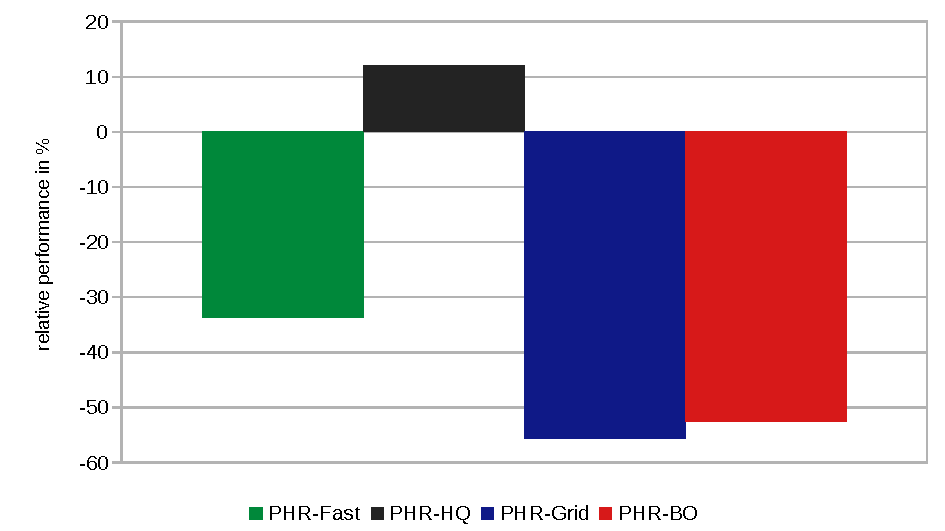
\includegraphics[width=300pt]{images/performance_difference.pdf}
    \caption{Relative difference to LBVH in percent.}
    \label{fig:difference}
\end{figure}
\subsection{Optimization Performance}
Figure \ref{fig:optimization} shows optimization times divided through average frame time, or in other words, how many frames could potentially be rendered instead of executing the optimization. Considering that the average performance increase of both methods amounted around 50\%, i.e. can potentially half the rendering time, optimizations start to become viable at half a frames duration and below. So even though the search space used in grid search is relatively low, the achieved times never reached what would be feasible in interactive applications. Bayesian optimization performed considerably better, but only reached competitive times in a few cases. Note that reaching this time does not equal a performance increase but just a hypothetical chance that frame times are increased. 

This shows that the presented optimization approaches still lack in performance and are not yet viable. PHR needs to be executed to evaluate the cost function, which is especially costly for parameters that result in high build times. This could be improved by limiting the search spacer further or making it dynamic and related to the scene's complexity. An interrupt after a maximum execution time might also be a solution. Bayesian optimization uses a costly run with maxed out parameters to determine the maximum build cost. This could be solved by reusing max values from previous optimizations. This topic is discussed further in section \ref{discussion_execute}.
\begin{figure}[H]
    \centering
    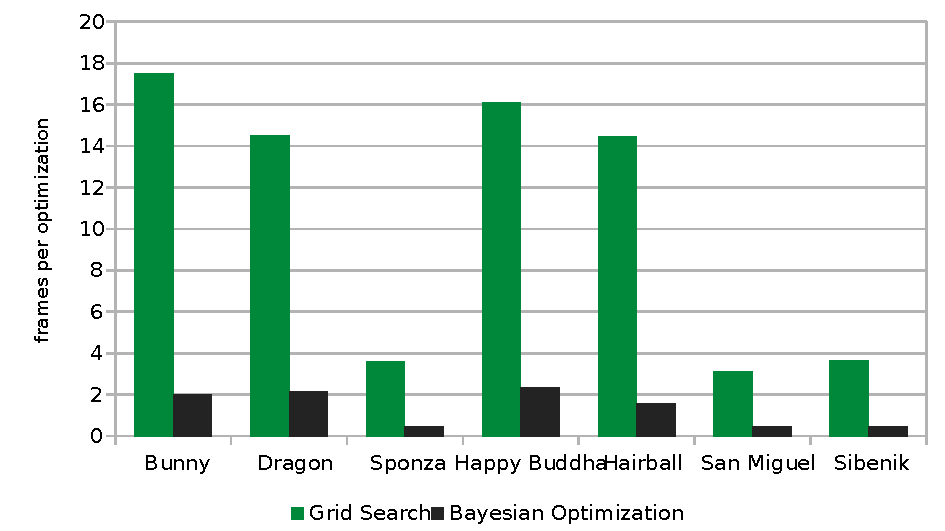
\includegraphics[width=300pt]{images/frame_per_optimization.pdf}
    \caption{Number of potential frames during optimization.}
    \label{fig:optimization}
\end{figure}
\clearpage
\begin{table}
\caption{Performance comparison of a representative selection of tested configuration at 256x256 resolution.}
\label{tab:frametime}
\centering
\begin{tabular}{ | c | m{3.5em} | m{3.5em} | m{3.5em} | m{3.5em} | m{3.5em} |  m{3.5em}|}
\hline
& build time (ms) & render time (ms) & frame time ms & build time (ms) & render time (ms) & frame time ms\\
\hline
& \multicolumn{1}{|m{4.5em}}{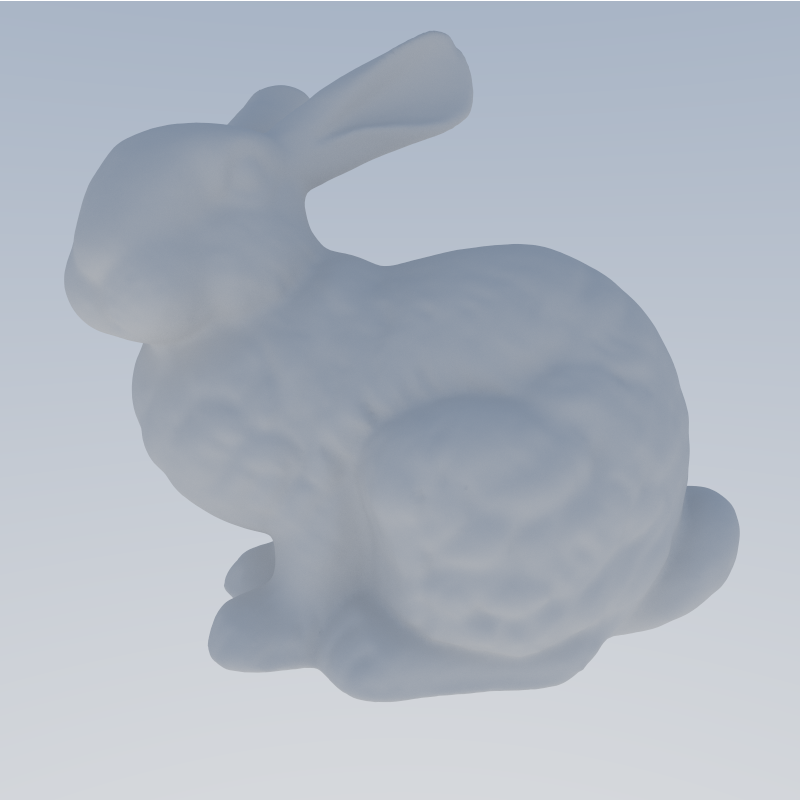
\includegraphics[width=60pt]{images/bunny.png}} &     \multicolumn{2}{m{4em}|}{Bunny \#triangles 144k} 
& \multicolumn{1}{|m{4.5em}}{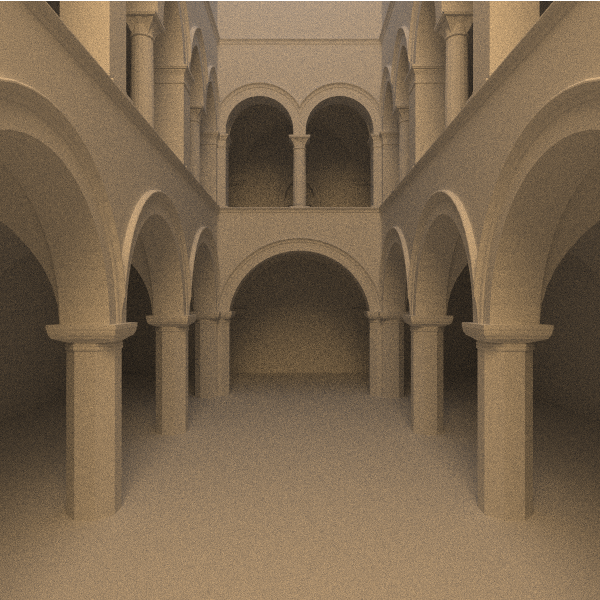
\includegraphics[width=60pt]{images/sponza.png}} & \multicolumn{2}{m{4em}|}{Sponza \#triangles 66k}\\
\hline
LBVH & 152.0 & 21.9 & 173.9            & 70.4 & 227.0 & 297.5 \\
PHR-Fast & 70.5 & 20.1 & 90.6          & 27.6 & 184 & 211.6 \\
PHR-HQ & 273.0 & 20.7 & 293.7          &  94.7 & 182 & 276.7\\
\hline
PHR-Grid & 14.4 & 20.8 & 35.2        &  17.2 & 207 & 224.2\\
PHR-BO & 14.2 & 20.7 & 34.97         &  21.7 & 200 & 221.7\\
\hline
& \multicolumn{1}{|m{4.5em}}{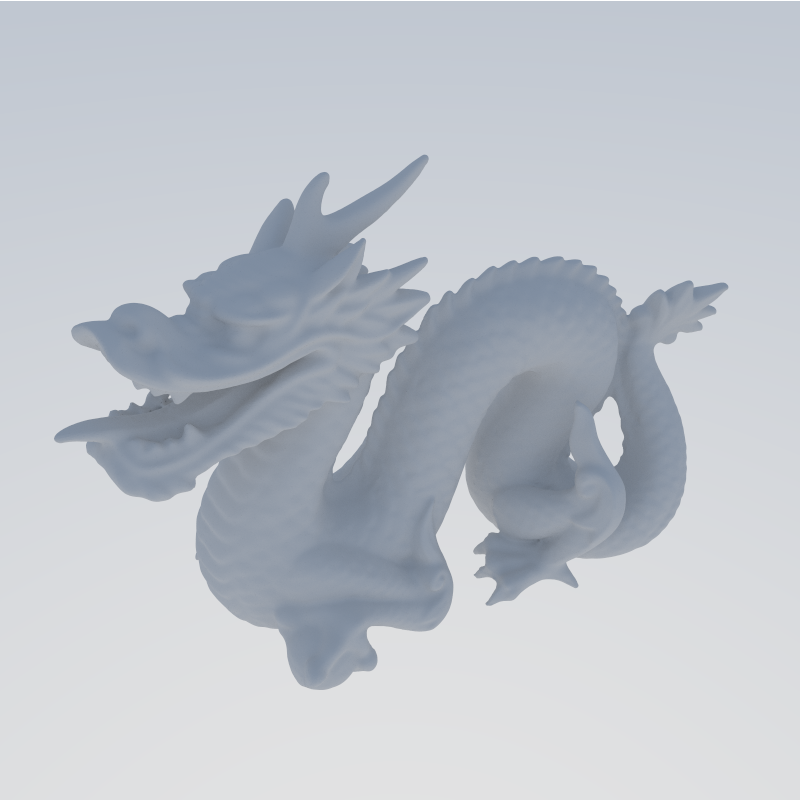
\includegraphics[width=60pt]{images/dragon.png}} &     \multicolumn{2}{m{4em}|}{Dragon \#triangles 817k}

& \multicolumn{1}{|m{4.5em}}{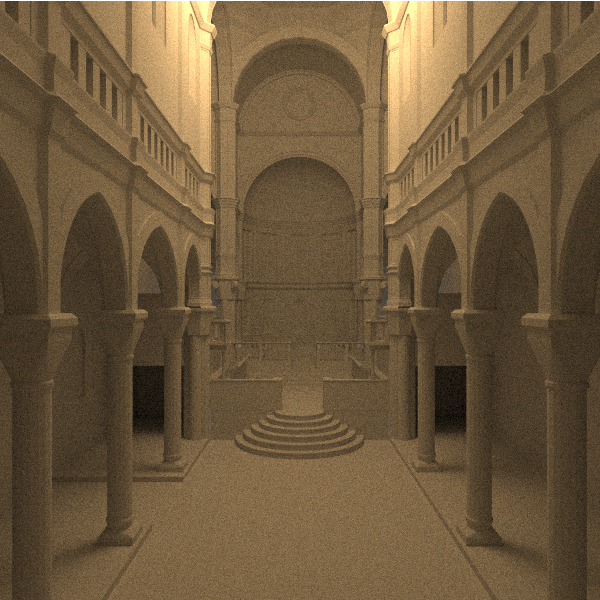
\includegraphics[width=60pt]{images/sibenik.png}} & \multicolumn{2}{m{4em}|}{Sibenik \#triangles 75k}\\

\hline
LBVH & 900.0 & 28.1 & 928.2              &  72.1 & 226.1 & 298.1\\
PHR-Fast & 150.0 & 32.5 & 182.5            &  32.5 & 205 & 237.5\\
PHR-HQ & 1090.0 & 29.0 & 1119.0              &  98.4 & 187  &285.4\\
\hline
PHR-Grid & 31.7 & 63.5 & 95.2            & 19.1 & 236 & 255.1  \\
PHR-BO & 30.8 & 66.1 & 96.9              & 28.1 & 220 & 248.1 \\
\hline
& \multicolumn{1}{|m{4.5em}}{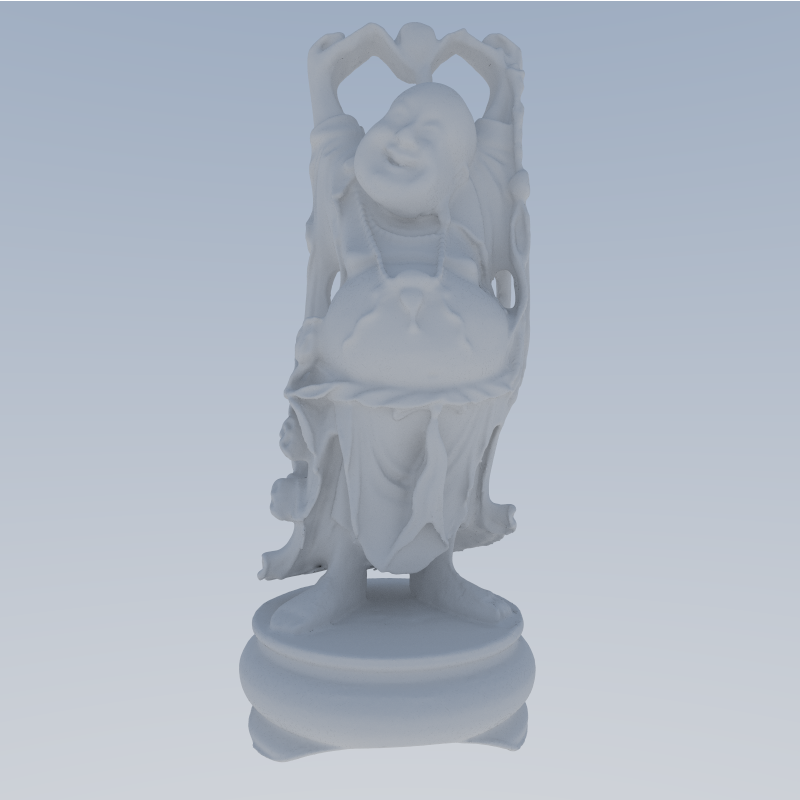
\includegraphics[width=60pt]{images/buddha.png}} & \multicolumn{2}{m{4em}|}{Happy Buddha \#triangles 1087k}

& \multicolumn{1}{|m{4.5em}}{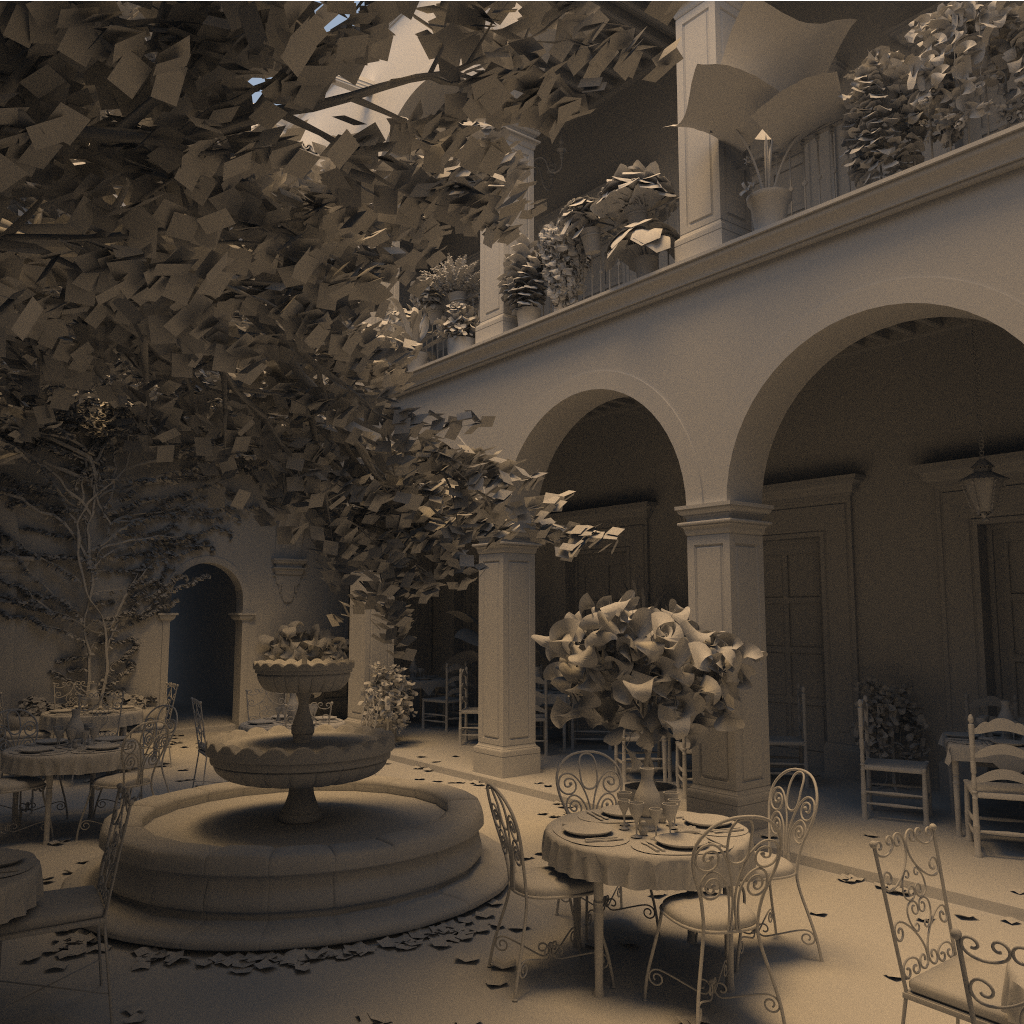
\includegraphics[width=60pt]{images/san_miguel.png}} &     \multicolumn{2}{m{4.5em}|}{San Miguel \#triangles 5617k}\\


\hline
LBVH & 1080 & 25 & 1105                    & 6010.0 & 816.0 & 6826.6 \\                   
PHR-Fast & 190 & 27.6 & 217.6                   & 432.0 & 7830.0 & 8262.0 \\
PHR-HQ & 1250 & 23.7 & 1273.7                     & 2600.0 & 812.3 & 3412.3 \\
\hline
PHR-Grid & 40.5 & 57.5 &98                   & 1300.0 & 1856.6 & 3156.6  \\
PHR-BO & 42.1 &58 &100.1                     & 815.0 & 3203.3 & 4018.3 \\
\hline
\end{tabular}
\end{table}
\cleardoublepage
\section{Discussion}


\section{Conclusion}

\subsection{Further Work}
Path tracing is a very extensive topic and especially considering the task of writing a complete path tracer, there is a lot of work left open. Considering the path tracer, a missing but essential aspect is denoising. As discussed earlier, recently a lot of progress has been achieved in that field of research and integrating some of that into this project would be an interesting addition. Importance sampling is another technique that was not considered in this work, but might improve it a decent amount. 
Staying with the main focus of this thesis, replacing LBVH with another fast BVH builder could bring interesting results. The full sweep SAH at the core of PHR is still relatively expensive and might be replacable by the more efficient binning SAH for better performance, or extended by using other cost functions like ray distribution heuristic or occlusion heuristic. Finally, optimization of PHRs hyperparameters is not ideal yet and might be improved by either using other optimization procedures, or improving the evaluation function.
\part*{Bibliography}
\addcontentsline{toc}{part}{Bibliography}
\nocite{*}
\bibliographystyle{apalike}
\bibliography{literatures/list}

\end{document}